\chapter{RS232 Modul}
\label{ch:rs232}
Dataforbindelse mellem SI og KI anvender en RS232-protokol, dette betyder at UART signalet fra SM skal level konverteres til RS232-protokol, nedenfor vises det overordnet blokdiagram for RS232 konverteren.
\begin{figure}[H]
\centering
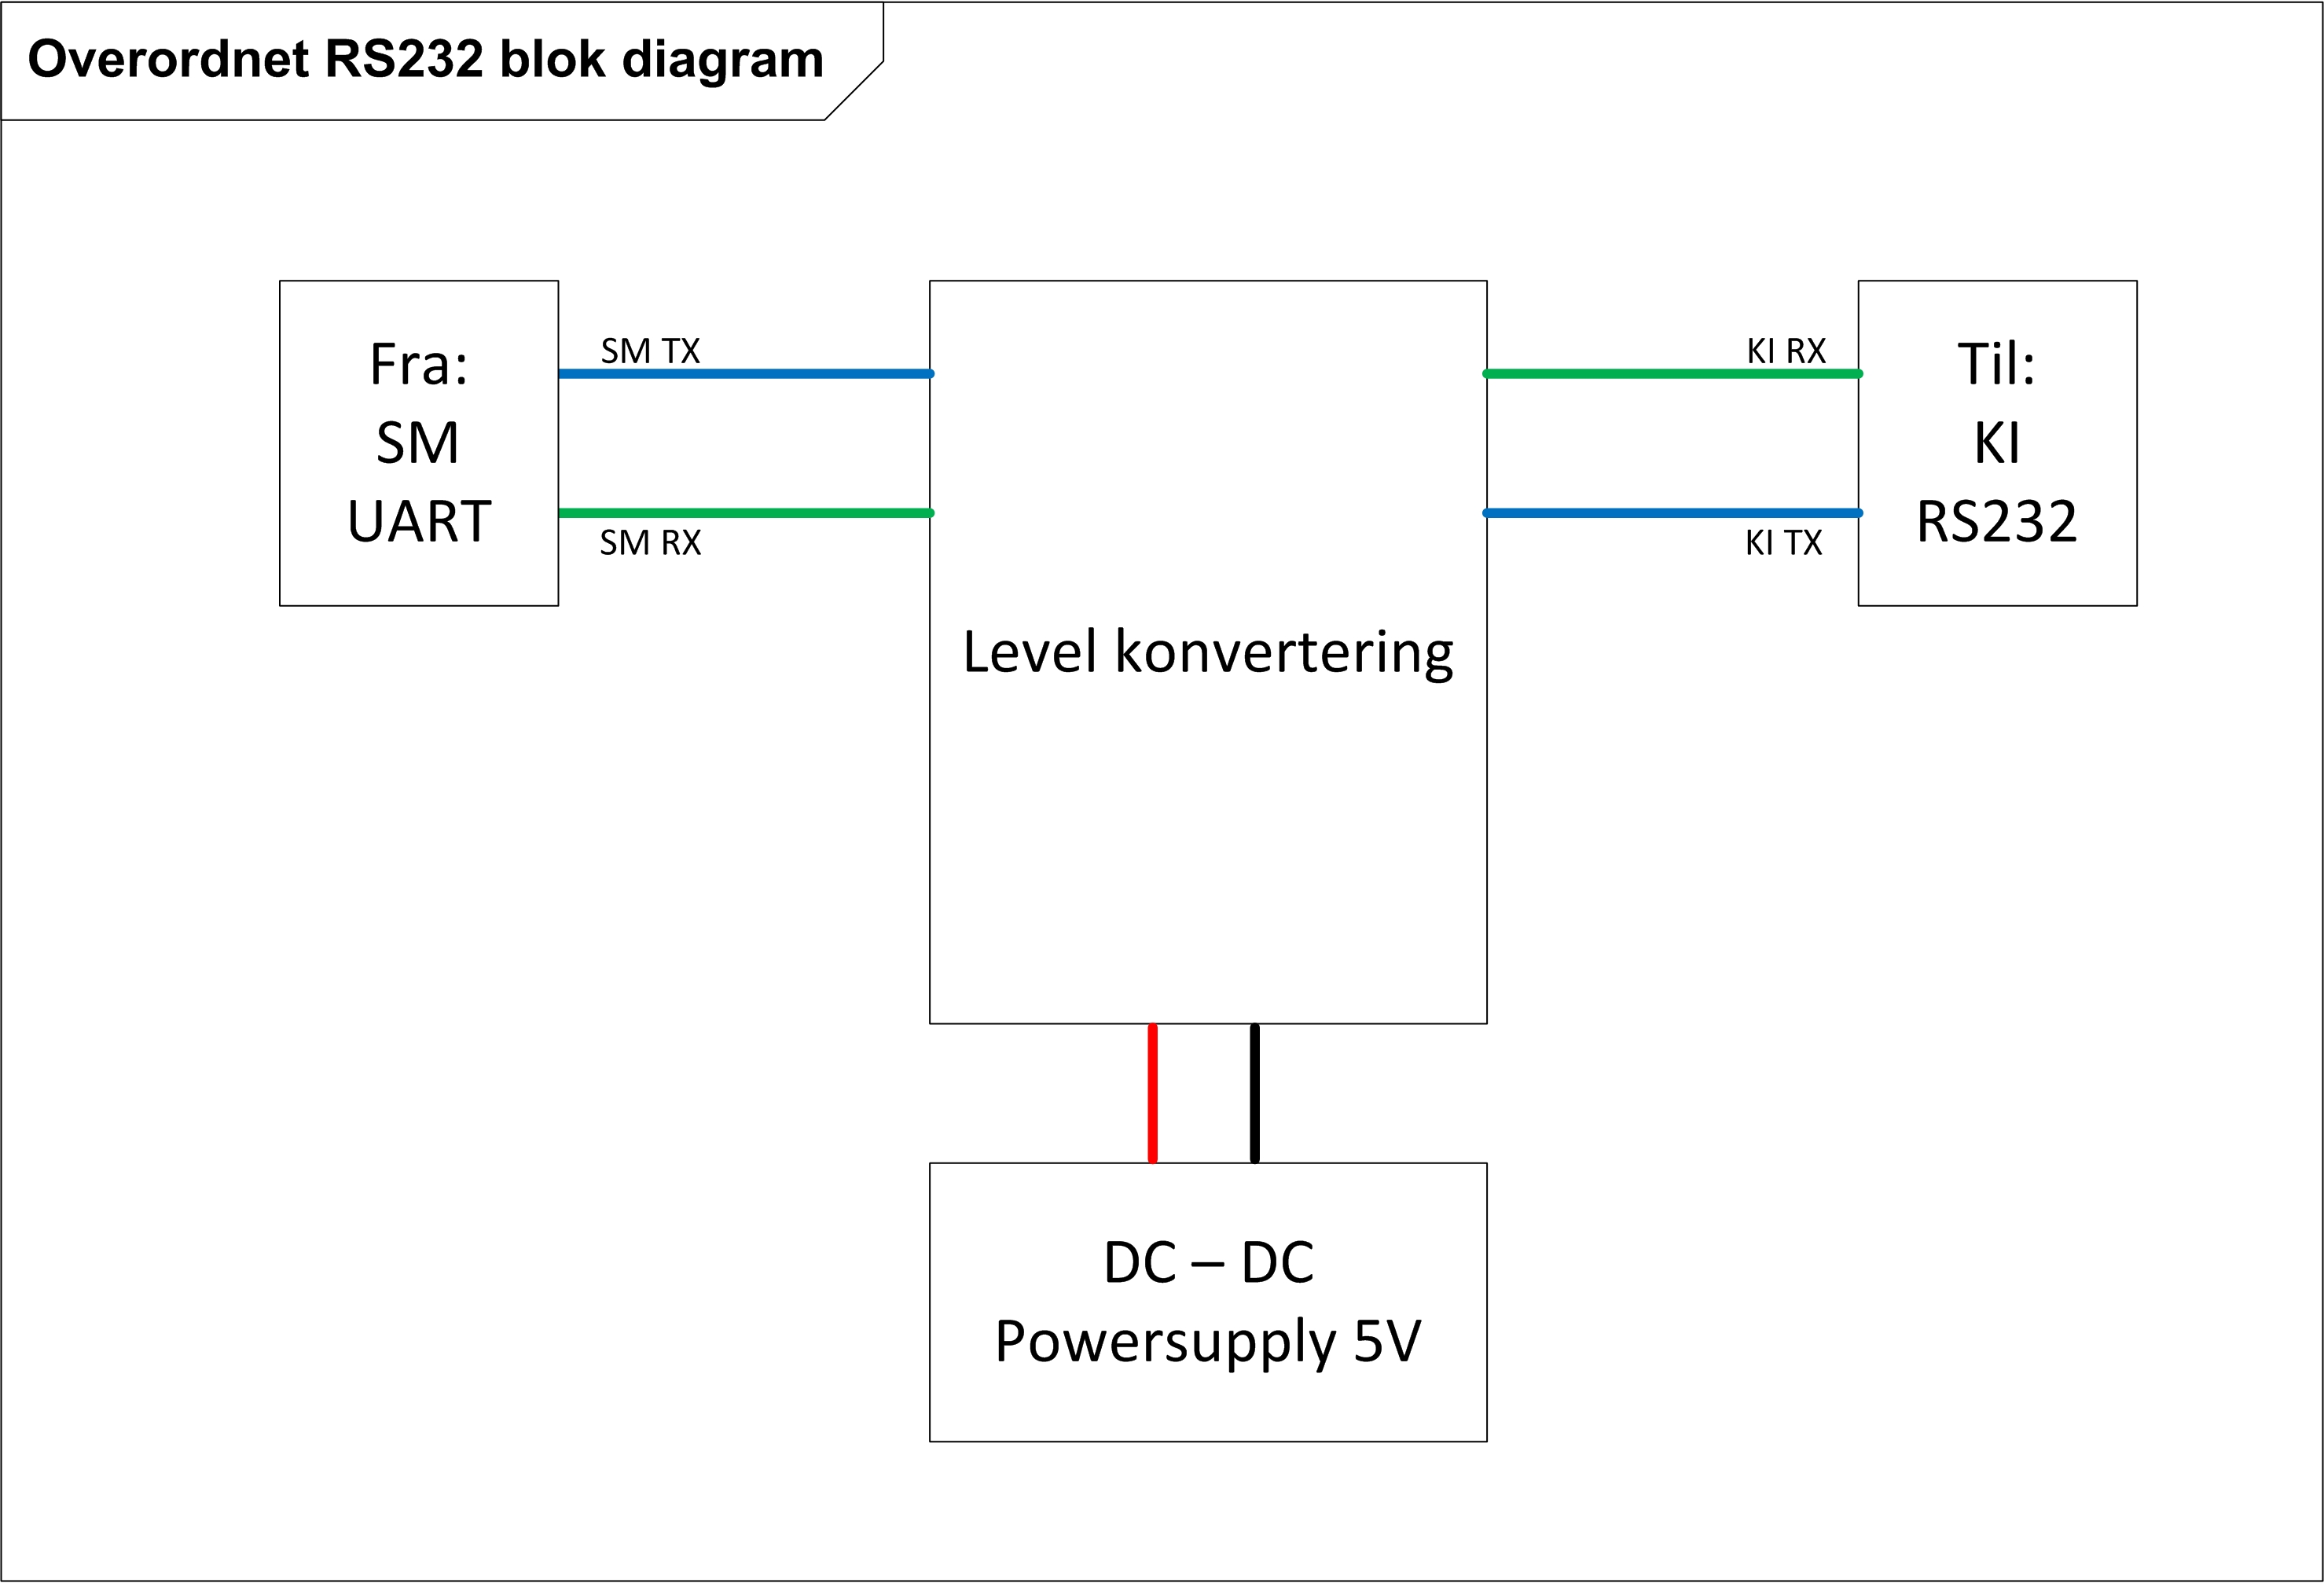
\includegraphics[width=0.5\textwidth]{billeder/RS232ModulBlok}
\caption{Blokdiagram for RS232ModulBlok}
\label{fig:RS232ModulBlok}
\end{figure}


\begin{figure}[H]
\centering
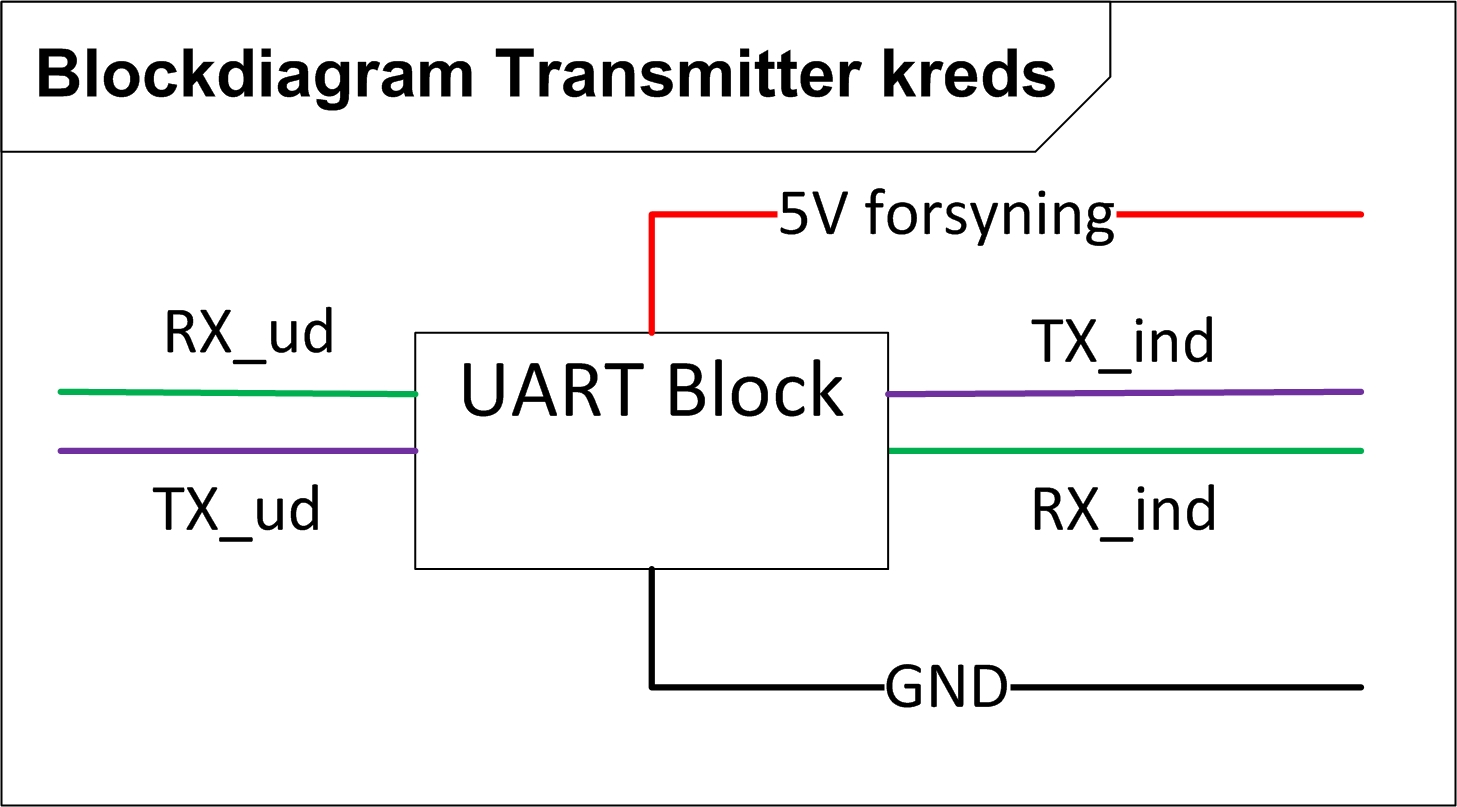
\includegraphics[width=0.5\textwidth]{billeder/uartblock}
\caption{Blokdiagram for Uart Block}
\label{fig:SMUART}
\end{figure}
\subsubsection{Signalbeskrivelser:}
For signalbeskrivelser se \textit{tabel~\ref{table:UARTSignalerSM}}
\begin{table}[H]
\begin{tabular}{|p{3cm}|p{3cm}|p{3cm}|p{4.5cm}|} \hline
\cellcolor[gray]{0.85}Signal navn& \cellcolor[gray]{0.85}Type &\cellcolor[gray]{0.85}Spænding&\cellcolor[gray]{0.85}Beskrivelse\\ \hline
TX\_ud & Analog & $\sim$0V til $\sim$5V & TX fra PSoC blokken.\\ \hline
RX\_ud & Analog & $\sim$0V til $\sim$5V & RX fra PSoC blokken. \\ \hline
TX\_ind & Analog & $\sim$0V til $\sim$5V & TX fra KI modulet.\\ \hline
RX\_ind & Analog & $\sim$0V til $\sim$5V & RX fra KI modulet. \\ \hline
5V forsyning & Analog DC & 5V$\pm$0.2V & 5V forsyning der leveres fra powersupplyen beskrevet under powersupply.\\ \hline
GND & Ground & 0V & Ground i systemet \\ \hline
\end{tabular}
\caption{Tabel over signaler i PSoC blokken}
\label{table:UARTSignalerSM}
\end{table}


For at SM kan få forbindelse med KI,   det er besluttet at bruge en RS232 dataforbindelse enheden fungere som en level konverter mellem SM og KI. 
\begin{figure}[H]
\centering
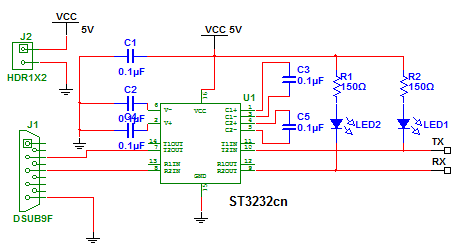
\includegraphics[scale=1]{billeder/HWUART}
\caption{Realisering for UART Block}
\label{fig:SMHWUARTB}
\end{figure}
RS232 konverteren er blevet implemeteret sammen med SM 
